\begin{figure}[!ht]
    \centering
    % \includegraphics{}
    \begin{minipage}{.45\textwidth}
        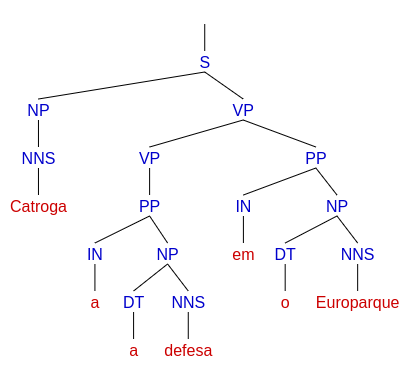
\includegraphics[width=\linewidth]{imagens/ec_cintil_sem_ponto_tree_trans.png}
        % \begin{forest}
        %     [
        %      [S 
        %       [NP 
        %       [NNS Catroga]
        %       ]
        %       [VP 
        %       [VP 
        %         [PP 
        %          [\textbf{IN a\_}]
        %          [NP 
        %           [\textbf{DT a}]
        %           [NNS defesa]
        %          ]
        %         ]
        %       ]
        %       [PP 
        %         [\textbf{IN em\_}]
        %         [NP 
        %          [\textbf{DT o}]
        %          [NNS Europarque]
        %         ]
        %       ]
        %       ]
        %      ]
        %     ]
        % \end{forest}
    \end{minipage}
    % 
    \begin{minipage}{.45\textwidth}
        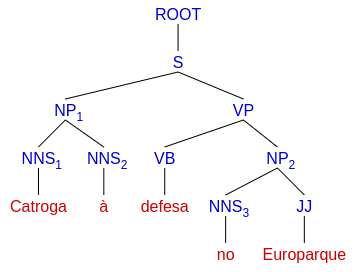
\includegraphics[width=\linewidth]{imagens/ec_cintil_sem_ponto_tree_sp.png}
        % \begin{forest}
        %     [ROOT
        %       [S
        %         [NP [NNS Catroga] [\textbf{JJ à}]]
        %         [VP [VB defesa]
        %           [NP [\textbf{NNS no}] [JJ Europarque]]]]]
        % \end{forest}
    \end{minipage}
    \caption[Estudo de caso CINTIL - Sentença transduzida sem pontuação]{Estudo da sentença eCTMP-000647/78121, \textquote{Catroga à defesa no Europarque}, que originalmente não possui nenhuma pontuação}
    \label{fig:ec_cintil_sem_ponto_tree}
\end{figure}